\documentclass[12pt]{extarticle}
\usepackage[letterpaper, left=0.75in, right=0.75in, top=0.8in, bottom=0.8in,
  headheight=20pt, headsep=16pt, footskip=30pt]{geometry}
\usepackage{fontspec}
\setmainfont{texgyreheros}[Extension=.otf, UprightFont=*-regular,
  BoldFont=*-bold, ItalicFont=*-italic, BoldItalicFont=*-bolditalic]
\usepackage{tikz}
\usetikzlibrary{shapes.geometric, arrows.meta}
\usepackage{array}
\usepackage{fancyhdr}
\pagestyle{fancy}
\fancyhf{}
\fancyhead[L]{Week 8 / Rook race and Nim / Grades 2--3}
\fancyfoot[L]{Bellingham Math Circle / Week 8 / F08-M-v4}
\fancyfoot[R]{\thepage}
\renewcommand{\headrulewidth}{0pt}
\setlength{\parindent}{0pt}
\setlength{\parskip}{0pt}
\linespread{1.12}
\hyphenpenalty=10000
\exhyphenpenalty=10000
\newcommand{\prob}[1]{\textbf{Problem #1:}}
\begin{document}
\raggedright
\noindent\begin{minipage}[c]{4.9in}\raggedright
Players take turns. On a board, a move slides the token straight left or straight down, toward the star's side, one or more squares. Whoever moves the token onto the star wins.

\vspace{0.12in}
In a game with piles of counters, a move takes one or more counters from one pile. Whoever takes the last counter wins.
\end{minipage}\hfill\begin{minipage}[c]{1.8in}\raggedleft
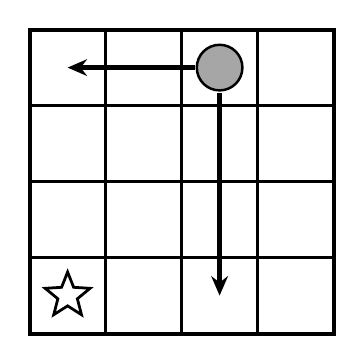
\begin{tikzpicture}[x=1in,y=1in]
\draw[line width=0.9pt] (0,0) grid[step=0.38] (1.5200,1.5200);
\draw[line width=1.4pt] (0,0) rectangle (1.5200,1.5200);
\node[star, star points=5, star point ratio=2.3, draw=black, line width=1.0pt, inner sep=0pt, outer sep=0pt, minimum size=0.236in] at (0.1900,0.1900) {};
\filldraw[fill=black!35, draw=black, line width=0.9pt] (0.9500,1.3300) circle (0.1140);
\draw[-{Stealth[length=7pt,width=6pt]}, line width=1.6pt] (0.8246,1.3300) -- (0.1900,1.3300);
\draw[-{Stealth[length=7pt,width=6pt]}, line width=1.6pt] (0.9500,1.2046) -- (0.9500,0.1900);
\end{tikzpicture}
\end{minipage}

\vspace{0.35in}
\prob{1} Play many games on a 5-by-5 board from each of these starting squares. Would you rather go first or second?

\vspace{0.3in}
\noindent \begin{minipage}[t]{3.35in}\centering
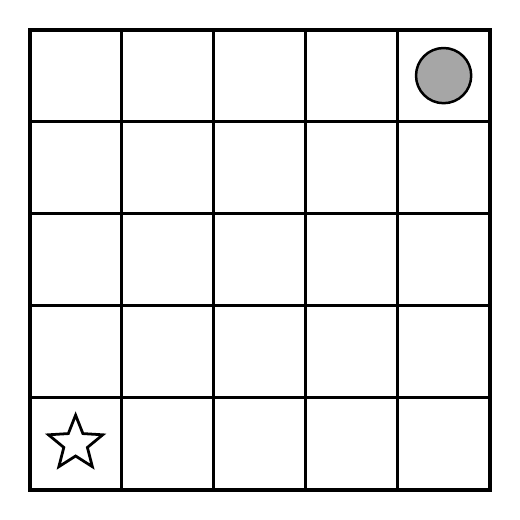
\begin{tikzpicture}[x=1in,y=1in]
\draw[line width=0.9pt] (0,0) grid[step=0.46] (2.3000,2.3000);
\draw[line width=1.4pt] (0,0) rectangle (2.3000,2.3000);
\node[star, star points=5, star point ratio=2.3, draw=black, line width=1.0pt, inner sep=0pt, outer sep=0pt, minimum size=0.285in] at (0.2300,0.2300) {};
\filldraw[fill=black!35, draw=black, line width=0.9pt] (2.0700,2.0700) circle (0.1380);
\end{tikzpicture}

\vspace{0.45in}
\begin{tikzpicture}[x=1in,y=1in]\draw[line width=0.6pt] (0,0) -- (1.8,0);\end{tikzpicture}
\end{minipage} \hfill \begin{minipage}[t]{3.35in}\centering
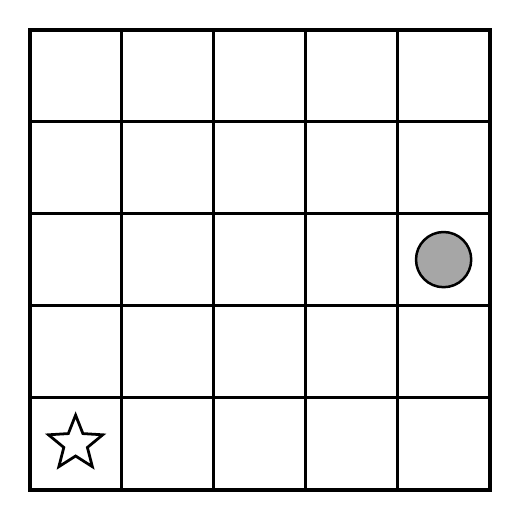
\begin{tikzpicture}[x=1in,y=1in]
\draw[line width=0.9pt] (0,0) grid[step=0.46] (2.3000,2.3000);
\draw[line width=1.4pt] (0,0) rectangle (2.3000,2.3000);
\node[star, star points=5, star point ratio=2.3, draw=black, line width=1.0pt, inner sep=0pt, outer sep=0pt, minimum size=0.285in] at (0.2300,0.2300) {};
\filldraw[fill=black!35, draw=black, line width=0.9pt] (2.0700,1.1500) circle (0.1380);
\end{tikzpicture}

\vspace{0.45in}
\begin{tikzpicture}[x=1in,y=1in]\draw[line width=0.6pt] (0,0) -- (1.8,0);\end{tikzpicture}
\end{minipage}

\vspace{0.4in}

\noindent \begin{minipage}[t]{3.35in}\centering
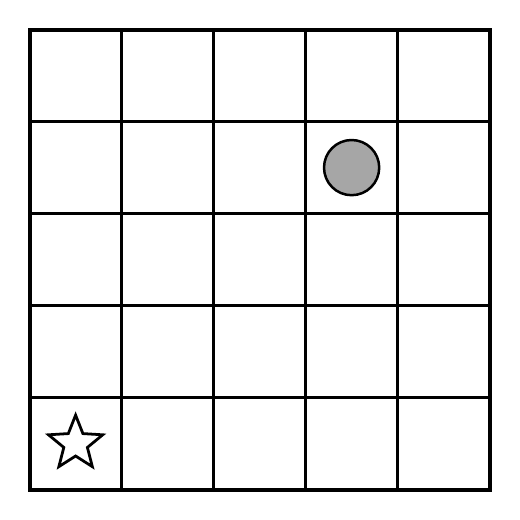
\begin{tikzpicture}[x=1in,y=1in]
\draw[line width=0.9pt] (0,0) grid[step=0.46] (2.3000,2.3000);
\draw[line width=1.4pt] (0,0) rectangle (2.3000,2.3000);
\node[star, star points=5, star point ratio=2.3, draw=black, line width=1.0pt, inner sep=0pt, outer sep=0pt, minimum size=0.285in] at (0.2300,0.2300) {};
\filldraw[fill=black!35, draw=black, line width=0.9pt] (1.6100,1.6100) circle (0.1380);
\end{tikzpicture}

\vspace{0.45in}
\begin{tikzpicture}[x=1in,y=1in]\draw[line width=0.6pt] (0,0) -- (1.8,0);\end{tikzpicture}
\end{minipage} \hfill \begin{minipage}[t]{3.35in}\centering
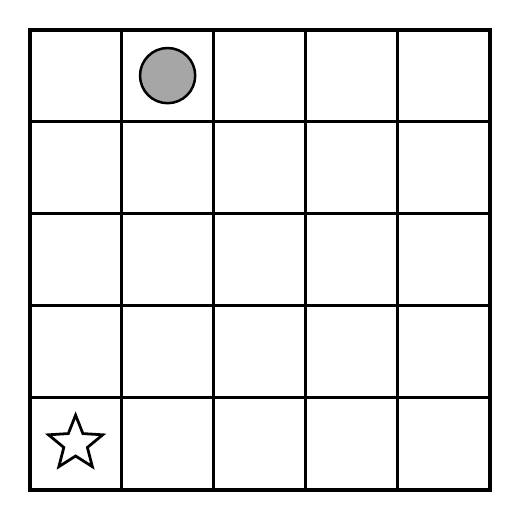
\begin{tikzpicture}[x=1in,y=1in]
\draw[line width=0.9pt] (0,0) grid[step=0.46] (2.3000,2.3000);
\draw[line width=1.4pt] (0,0) rectangle (2.3000,2.3000);
\node[star, star points=5, star point ratio=2.3, draw=black, line width=1.0pt, inner sep=0pt, outer sep=0pt, minimum size=0.285in] at (0.2300,0.2300) {};
\filldraw[fill=black!35, draw=black, line width=0.9pt] (0.6900,2.0700) circle (0.1380);
\end{tikzpicture}

\vspace{0.45in}
\begin{tikzpicture}[x=1in,y=1in]\draw[line width=0.6pt] (0,0) -- (1.8,0);\end{tikzpicture}
\end{minipage}
\newpage
\prob{2} Color every square of this 8-by-8 board except the star. Color a square green if you would rather go first when the token starts there, and red if you would rather go second.

\vspace{0.25in}
\begin{center}
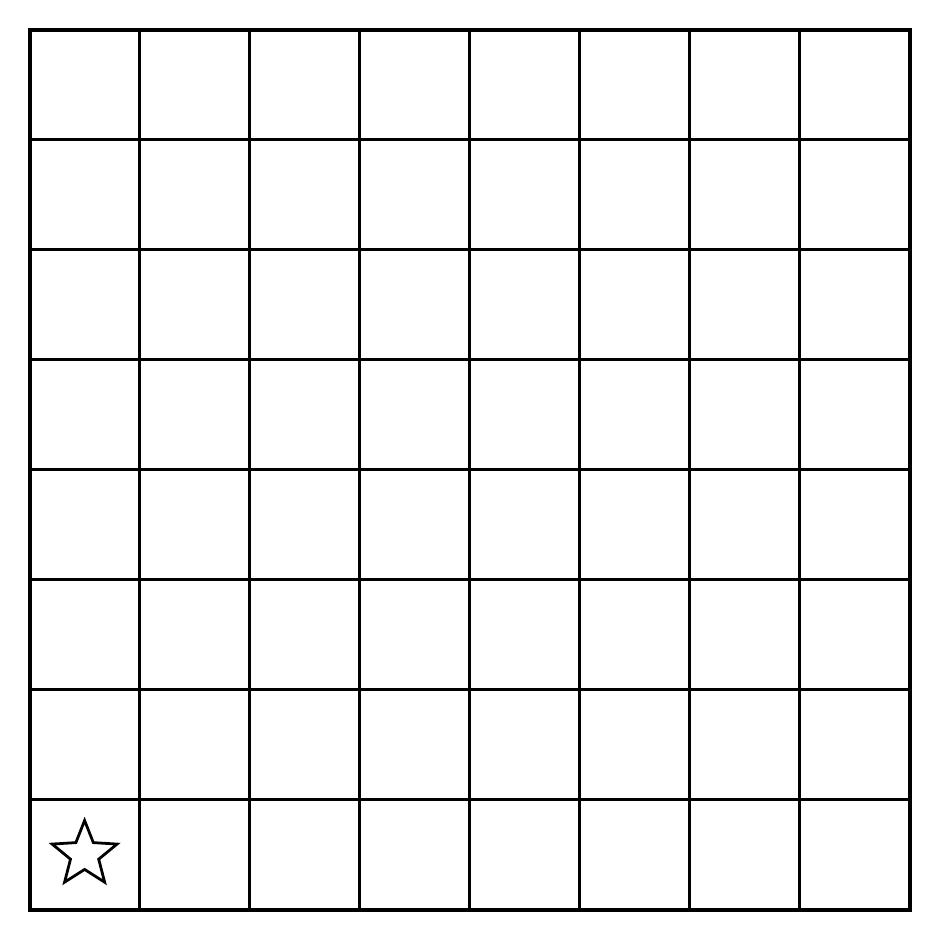
\begin{tikzpicture}[x=1in,y=1in]
\draw[line width=0.9pt] (0,0) grid[step=0.55] (4.4000,4.4000);
\draw[line width=1.4pt] (0,0) rectangle (4.4000,4.4000);
\node[star, star points=5, star point ratio=2.3, draw=black, line width=1.0pt, inner sep=0pt, outer sep=0pt, minimum size=0.341in] at (0.2750,0.2750) {};
\end{tikzpicture}
\end{center}
\vspace{0.35in}

\noindent\begin{minipage}[t]{4.5in}\vspace{0pt}\raggedright
\prob{3} Your partner goes first, with the token in the top-right corner of an 8-by-8 board. Explain how you can always win, however your partner moves.
\end{minipage}\hfill\begin{minipage}[t]{2.2in}\vspace{0pt}\raggedleft
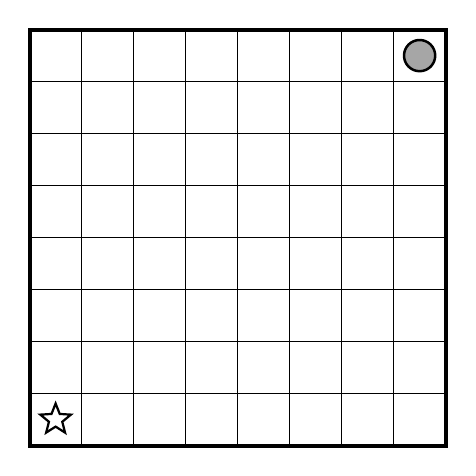
\begin{tikzpicture}[x=1in,y=1in]
\draw[line width=0.6pt] (0,0) grid[step=0.26] (2.0800,2.0800);
\draw[line width=1.4pt] (0,0) rectangle (2.0800,2.0800);
\node[star, star points=5, star point ratio=2.3, draw=black, line width=0.8pt, inner sep=0pt, outer sep=0pt, minimum size=0.161in] at (0.1300,0.1300) {};
\filldraw[fill=black!35, draw=black, line width=0.9pt] (1.9500,1.9500) circle (0.0780);
\end{tikzpicture}
\end{minipage}

\newpage
\prob{4} Play many games with two piles of counters from each start. Would you rather go first or second?

\vspace{0.3in}
\noindent \begin{minipage}[b]{1.55in}\centering
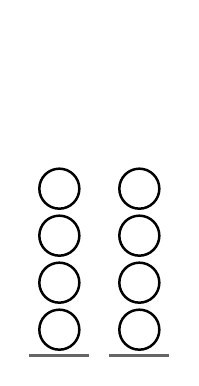
\begin{tikzpicture}[x=1in,y=1in]
\path (0,-0.03) -- (0,1.6100);
\draw[line width=0.9pt, fill=white] (0.0000,0.1000) circle (0.1000);
\draw[line width=0.9pt, fill=white] (0.0000,0.3350) circle (0.1000);
\draw[line width=0.9pt, fill=white] (0.0000,0.5700) circle (0.1000);
\draw[line width=0.9pt, fill=white] (0.0000,0.8050) circle (0.1000);
\draw[line width=1.2pt, black!60] (-0.1500,-0.03) -- (0.1500,-0.03);
\draw[line width=0.9pt, fill=white] (0.4000,0.1000) circle (0.1000);
\draw[line width=0.9pt, fill=white] (0.4000,0.3350) circle (0.1000);
\draw[line width=0.9pt, fill=white] (0.4000,0.5700) circle (0.1000);
\draw[line width=0.9pt, fill=white] (0.4000,0.8050) circle (0.1000);
\draw[line width=1.2pt, black!60] (0.2500,-0.03) -- (0.5500,-0.03);
\end{tikzpicture}

\vspace{0.12in}4 and 4

\vspace{0.35in}\begin{tikzpicture}[x=1in,y=1in]\draw[line width=0.6pt] (0,0) -- (1.3,0);\end{tikzpicture}
\end{minipage}\hfill\begin{minipage}[b]{1.55in}\centering
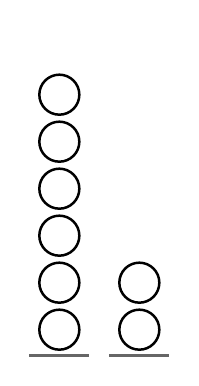
\begin{tikzpicture}[x=1in,y=1in]
\path (0,-0.03) -- (0,1.6100);
\draw[line width=0.9pt, fill=white] (0.0000,0.1000) circle (0.1000);
\draw[line width=0.9pt, fill=white] (0.0000,0.3350) circle (0.1000);
\draw[line width=0.9pt, fill=white] (0.0000,0.5700) circle (0.1000);
\draw[line width=0.9pt, fill=white] (0.0000,0.8050) circle (0.1000);
\draw[line width=0.9pt, fill=white] (0.0000,1.0400) circle (0.1000);
\draw[line width=0.9pt, fill=white] (0.0000,1.2750) circle (0.1000);
\draw[line width=1.2pt, black!60] (-0.1500,-0.03) -- (0.1500,-0.03);
\draw[line width=0.9pt, fill=white] (0.4000,0.1000) circle (0.1000);
\draw[line width=0.9pt, fill=white] (0.4000,0.3350) circle (0.1000);
\draw[line width=1.2pt, black!60] (0.2500,-0.03) -- (0.5500,-0.03);
\end{tikzpicture}

\vspace{0.12in}6 and 2

\vspace{0.35in}\begin{tikzpicture}[x=1in,y=1in]\draw[line width=0.6pt] (0,0) -- (1.3,0);\end{tikzpicture}
\end{minipage}\hfill\begin{minipage}[b]{1.55in}\centering
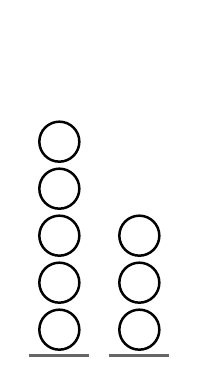
\begin{tikzpicture}[x=1in,y=1in]
\path (0,-0.03) -- (0,1.6100);
\draw[line width=0.9pt, fill=white] (0.0000,0.1000) circle (0.1000);
\draw[line width=0.9pt, fill=white] (0.0000,0.3350) circle (0.1000);
\draw[line width=0.9pt, fill=white] (0.0000,0.5700) circle (0.1000);
\draw[line width=0.9pt, fill=white] (0.0000,0.8050) circle (0.1000);
\draw[line width=0.9pt, fill=white] (0.0000,1.0400) circle (0.1000);
\draw[line width=1.2pt, black!60] (-0.1500,-0.03) -- (0.1500,-0.03);
\draw[line width=0.9pt, fill=white] (0.4000,0.1000) circle (0.1000);
\draw[line width=0.9pt, fill=white] (0.4000,0.3350) circle (0.1000);
\draw[line width=0.9pt, fill=white] (0.4000,0.5700) circle (0.1000);
\draw[line width=1.2pt, black!60] (0.2500,-0.03) -- (0.5500,-0.03);
\end{tikzpicture}

\vspace{0.12in}5 and 3

\vspace{0.35in}\begin{tikzpicture}[x=1in,y=1in]\draw[line width=0.6pt] (0,0) -- (1.3,0);\end{tikzpicture}
\end{minipage}\hfill\begin{minipage}[b]{1.55in}\centering
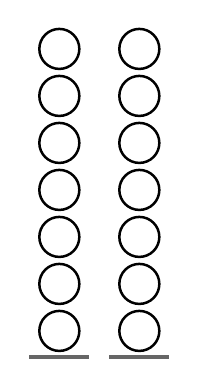
\begin{tikzpicture}[x=1in,y=1in]
\path (0,-0.03) -- (0,1.6100);
\draw[line width=0.9pt, fill=white] (0.0000,0.1000) circle (0.1000);
\draw[line width=0.9pt, fill=white] (0.0000,0.3350) circle (0.1000);
\draw[line width=0.9pt, fill=white] (0.0000,0.5700) circle (0.1000);
\draw[line width=0.9pt, fill=white] (0.0000,0.8050) circle (0.1000);
\draw[line width=0.9pt, fill=white] (0.0000,1.0400) circle (0.1000);
\draw[line width=0.9pt, fill=white] (0.0000,1.2750) circle (0.1000);
\draw[line width=0.9pt, fill=white] (0.0000,1.5100) circle (0.1000);
\draw[line width=1.2pt, black!60] (-0.1500,-0.03) -- (0.1500,-0.03);
\draw[line width=0.9pt, fill=white] (0.4000,0.1000) circle (0.1000);
\draw[line width=0.9pt, fill=white] (0.4000,0.3350) circle (0.1000);
\draw[line width=0.9pt, fill=white] (0.4000,0.5700) circle (0.1000);
\draw[line width=0.9pt, fill=white] (0.4000,0.8050) circle (0.1000);
\draw[line width=0.9pt, fill=white] (0.4000,1.0400) circle (0.1000);
\draw[line width=0.9pt, fill=white] (0.4000,1.2750) circle (0.1000);
\draw[line width=0.9pt, fill=white] (0.4000,1.5100) circle (0.1000);
\draw[line width=1.2pt, black!60] (0.2500,-0.03) -- (0.5500,-0.03);
\end{tikzpicture}

\vspace{0.12in}7 and 7

\vspace{0.35in}\begin{tikzpicture}[x=1in,y=1in]\draw[line width=0.6pt] (0,0) -- (1.3,0);\end{tikzpicture}
\end{minipage}
\vspace{0.6in}

\noindent\begin{minipage}[t]{3.3in}\vspace{0pt}\raggedright
\prob{5} Which two piles of counters make the same game as this 8-by-8 board with the token on the dot? Explain how each move on the board matches a move with the piles.
\end{minipage}\hfill\begin{minipage}[t]{3.3in}\vspace{0pt}\raggedleft
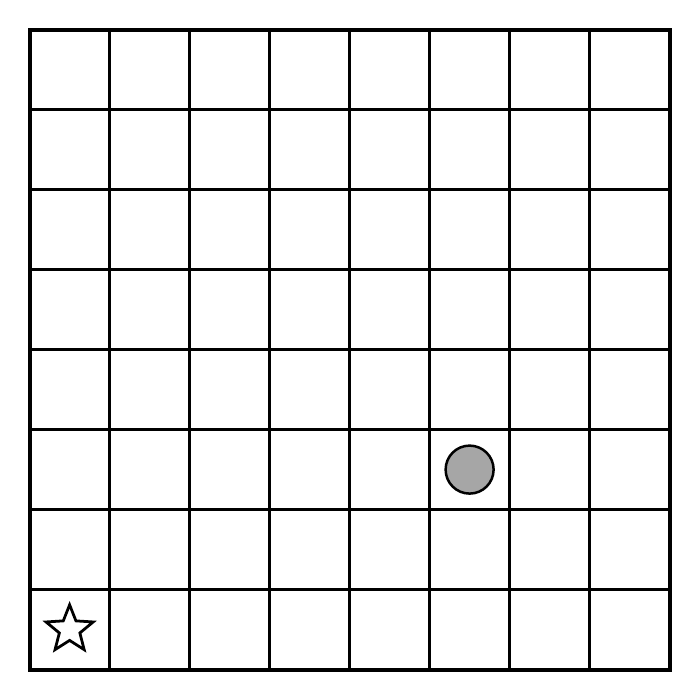
\begin{tikzpicture}[x=1in,y=1in]
\draw[line width=0.9pt] (0,0) grid[step=0.4] (3.2000,3.2000);
\draw[line width=1.4pt] (0,0) rectangle (3.2000,3.2000);
\node[star, star points=5, star point ratio=2.3, draw=black, line width=1.0pt, inner sep=0pt, outer sep=0pt, minimum size=0.248in] at (0.2000,0.2000) {};
\filldraw[fill=black!35, draw=black, line width=0.9pt] (2.2000,1.0000) circle (0.1200);
\end{tikzpicture}
\end{minipage}

\newpage
\prob{6} A game starts with piles of 52 and 37 counters. Would you rather go first or second? Explain how you can always win, however the other player moves.

\vspace{3.9in}

\prob{7} Play many games with three piles from each start. Would you rather go first or second?

\vspace{0.3in}
\noindent \begin{minipage}[b]{1.55in}\centering
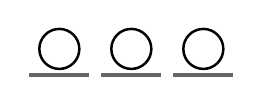
\begin{tikzpicture}[x=1in,y=1in]
\draw[line width=0.9pt, fill=white] (0.0000,0.1000) circle (0.1000);
\draw[line width=1.2pt, black!60] (-0.1500,-0.03) -- (0.1500,-0.03);
\draw[line width=0.9pt, fill=white] (0.3600,0.1000) circle (0.1000);
\draw[line width=1.2pt, black!60] (0.2100,-0.03) -- (0.5100,-0.03);
\draw[line width=0.9pt, fill=white] (0.7200,0.1000) circle (0.1000);
\draw[line width=1.2pt, black!60] (0.5700,-0.03) -- (0.8700,-0.03);
\end{tikzpicture}

\vspace{0.12in}1, 1, 1

\vspace{0.35in}\begin{tikzpicture}[x=1in,y=1in]\draw[line width=0.6pt] (0,0) -- (1.3,0);\end{tikzpicture}
\end{minipage}\hfill\begin{minipage}[b]{1.55in}\centering
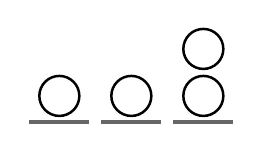
\begin{tikzpicture}[x=1in,y=1in]
\draw[line width=0.9pt, fill=white] (0.0000,0.1000) circle (0.1000);
\draw[line width=1.2pt, black!60] (-0.1500,-0.03) -- (0.1500,-0.03);
\draw[line width=0.9pt, fill=white] (0.3600,0.1000) circle (0.1000);
\draw[line width=1.2pt, black!60] (0.2100,-0.03) -- (0.5100,-0.03);
\draw[line width=0.9pt, fill=white] (0.7200,0.1000) circle (0.1000);
\draw[line width=0.9pt, fill=white] (0.7200,0.3350) circle (0.1000);
\draw[line width=1.2pt, black!60] (0.5700,-0.03) -- (0.8700,-0.03);
\end{tikzpicture}

\vspace{0.12in}1, 1, 2

\vspace{0.35in}\begin{tikzpicture}[x=1in,y=1in]\draw[line width=0.6pt] (0,0) -- (1.3,0);\end{tikzpicture}
\end{minipage}\hfill\begin{minipage}[b]{1.55in}\centering
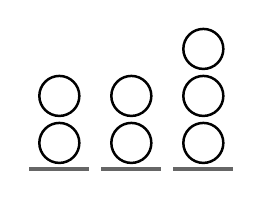
\begin{tikzpicture}[x=1in,y=1in]
\draw[line width=0.9pt, fill=white] (0.0000,0.1000) circle (0.1000);
\draw[line width=0.9pt, fill=white] (0.0000,0.3350) circle (0.1000);
\draw[line width=1.2pt, black!60] (-0.1500,-0.03) -- (0.1500,-0.03);
\draw[line width=0.9pt, fill=white] (0.3600,0.1000) circle (0.1000);
\draw[line width=0.9pt, fill=white] (0.3600,0.3350) circle (0.1000);
\draw[line width=1.2pt, black!60] (0.2100,-0.03) -- (0.5100,-0.03);
\draw[line width=0.9pt, fill=white] (0.7200,0.1000) circle (0.1000);
\draw[line width=0.9pt, fill=white] (0.7200,0.3350) circle (0.1000);
\draw[line width=0.9pt, fill=white] (0.7200,0.5700) circle (0.1000);
\draw[line width=1.2pt, black!60] (0.5700,-0.03) -- (0.8700,-0.03);
\end{tikzpicture}

\vspace{0.12in}2, 2, 3

\vspace{0.35in}\begin{tikzpicture}[x=1in,y=1in]\draw[line width=0.6pt] (0,0) -- (1.3,0);\end{tikzpicture}
\end{minipage}\hfill\begin{minipage}[b]{1.55in}\centering
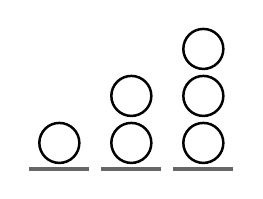
\begin{tikzpicture}[x=1in,y=1in]
\draw[line width=0.9pt, fill=white] (0.0000,0.1000) circle (0.1000);
\draw[line width=1.2pt, black!60] (-0.1500,-0.03) -- (0.1500,-0.03);
\draw[line width=0.9pt, fill=white] (0.3600,0.1000) circle (0.1000);
\draw[line width=0.9pt, fill=white] (0.3600,0.3350) circle (0.1000);
\draw[line width=1.2pt, black!60] (0.2100,-0.03) -- (0.5100,-0.03);
\draw[line width=0.9pt, fill=white] (0.7200,0.1000) circle (0.1000);
\draw[line width=0.9pt, fill=white] (0.7200,0.3350) circle (0.1000);
\draw[line width=0.9pt, fill=white] (0.7200,0.5700) circle (0.1000);
\draw[line width=1.2pt, black!60] (0.5700,-0.03) -- (0.8700,-0.03);
\end{tikzpicture}

\vspace{0.12in}1, 2, 3

\vspace{0.35in}\begin{tikzpicture}[x=1in,y=1in]\draw[line width=0.6pt] (0,0) -- (1.3,0);\end{tikzpicture}
\end{minipage}
\newpage
\prob{8} Find every start with three piles, each with 1, 2 or 3 counters, where you would rather go second. The order of the piles does not matter. Explain how you know you have found them all.

\vspace{4.1in}

\prob{9} Find all the starts with three piles, each with 1 to 6 counters, where you would rather go second. The order of the piles does not matter.

\end{document}
